\cleardoubleoddstandardpage
\chapter{Introduction}
This thesis aims to provide insights into the representations learned by \textsf{Graph Neural Networks} (\gnns). In this chapter, we will discuss the significance of graphs and how \gnns play a crucial role in analyzing them. We will present the motivation behind this work, the methods employed to gain insights, and an overview of the structure of this thesis.

\section{Motivation}
Graphs are ubiquitous in various fields of life. Despite not always being explicitly identified as such, the graph data model's flexibility and simplicity make it an effective tool for modeling a diverse range of data. Examples of graph modeling applications include unexpected instances, such as modeling text or images as a graph, as well as more complex instances like chemical molecules, citation networks, or connectivity encodings of the World Wide Web \cite{Mor+2020, Sca+2009}.

Although machine learning has achieved remarkable success with image classification (e.g., \cite{Zoph2018, He2016}) and text generation (e.g., \cite{Radford2019, Brown2020}) in the last decade, the lack of a significant breakthrough in machine learning for graphs can be attributed to the graph data model's inherent flexibility and simplicity. While, for example, an image classifier constrains its input data to be a grid-like image or a text generator expects its input to be a linear sequence of words, machine learning models working on graphs cannot leverage any constraints on the format or size of their input graphs without limiting their generality. 

To put this flexibility of the graph data model into perspective and give an idea of how ubiquitous graphs are in various fields, we refer back to the examples of image classifiers and text generators and demonstrate how seemingly natural the graph data model can encode their input data. For example, images can be encoded by a graph, such that each pixel of the image corresponds to a node in the graph holding its color value, and each node is connected to its neighboring pixel nodes. Similarly, for sequential data like text files, one can encode a directed graph where each word in this file is represented as a node with the word as a feature and connected outgoingly to the next following word. See \cref{fig:example_encodings} for an illustrative example of these encodings.

In recent years, a significant amount of research has been conducted to investigate \textsf{Graph Neural Networks} (\gnns). Among the most promising approaches are those utilizing the message-passing architecture, which was introduced by \cite{Sca+2009} and \cite{Gil+2017}. 
Empirically, this framework has demonstrated strong performance across various applications \cite{Kip+2017, Ham+2017, Xu2018}. However, its expressiveness is limited, as has been proven by the works of \cite{Morris2018}, as well as \cite{Xu2018}. These works establish a connection to the \textsf{Weisfeiler-Leman}\footnote{Based on \href{https://www.iti.zcu.cz/wl2018/pdf/leman.pdf}{https://www.iti.zcu.cz/wl2018/pdf/leman.pdf}, we will use the spelling ``Leman'' here, as requested by A. Leman, the co-inventor of the algorithm.} algorithm (\wl), originally proposed by \cite{Wei+1968} as a simple heuristic for the graph isomorphism problem. In particular, it has been proven that a \gnn based on the message-passing architecture can, at most, be as good as the \wl algorithm in distinguishing non-isomorphic graphs. Furthermore, the \wl method demonstrates numerous similarities with the fundamental workings of the \gnn architecture. It is, therefore, commonly believed that both methods are, to some extent, equivalent in their capacity to capture information in a graph.

Despite the remarkable empirical performance of \gnns, particularly compared to conventional graph kernel functions \cite{Mor+2020}, and the theoretical understanding of their ability to distinguish non-isomorphic graphs, there remains a limited understanding of the learned representations that drive this empirical success. This work aims to delve into these representations, seeking deeper insights into the factors contributing to the efficacy of \gnns.

\begin{figure}[!t]
 \centering
 \begin{subfigure}[b]{0.475\textwidth}
    \centering
    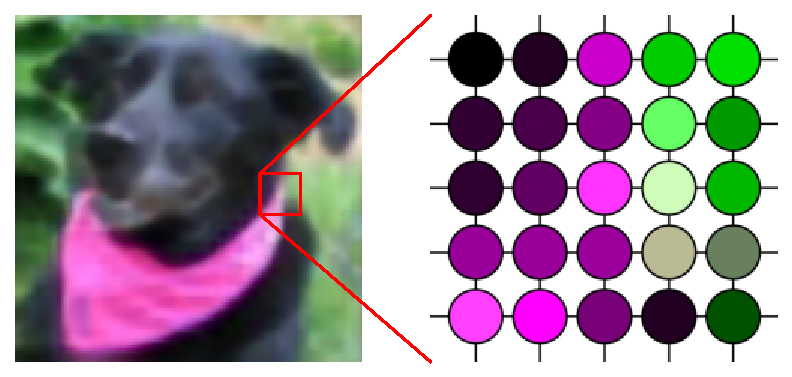
\includegraphics[width=\textwidth]{Figures/encoding_example.pdf}
    \caption{Graph Encoding of an Image\footnotemark}
 \end{subfigure}
 \hfill
 \begin{subfigure}[b]{0.475\textwidth}
    \centering
    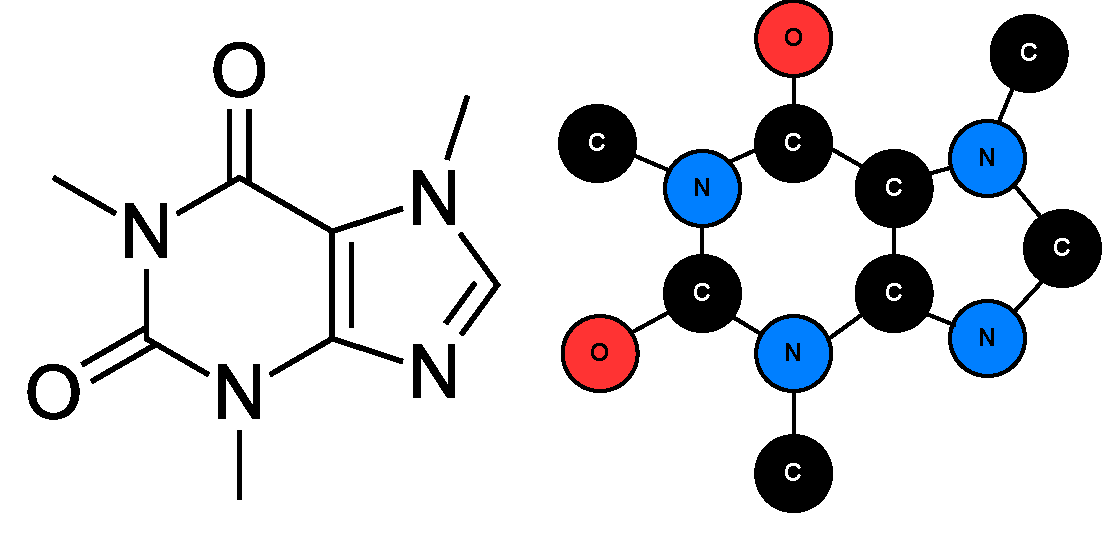
\includegraphics[width=\textwidth]{Figures/Example_Encoding_Molecule.pdf}
    \caption{Graph Encoding of a Molecule\footnotemark}
 \end{subfigure}
 \par\medskip
 \begin{subfigure}[b]{0.475\textwidth}
    \centering
    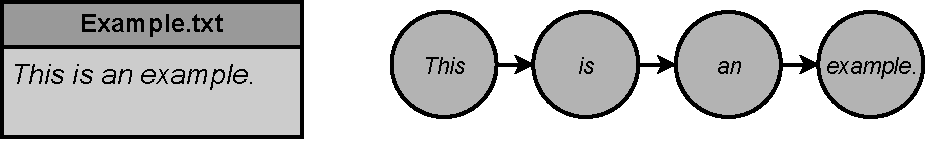
\includegraphics[width=\textwidth]{Figures/Example_Encoding_Text.pdf}
    \caption{Graph Encoding of a Text File.}
 \end{subfigure}
 \caption[Caption for LOF]{An overview of three examples of how graphs can be used to encode information across different domains. For each example, the conventional domain-specific encodings are visualized on the left, while on the right, we showcase how a graph can encode the same information. Note that these examples are just a sample; in actual practice, more detailed encodings are usually utilized to capture additional information.\footnotemark}
 \label{fig:example_encodings}
\end{figure}
\footnotetext[2]{The image of a dog is from the CIFAR-10 collection made available by \cite{Krizhevsky2009}.}
\footnotetext[3]{The illustration of the skeletal formula of caffeine is taken from \href{https://commons.wikimedia.org/wiki/File:Caffeine_structure.svg}{https://commons.wikimedia.org}.}
\footnotetext{All graphics were created using the free open source platform \href{https://www.draw.io}{https://www.draw.io}.}

\section{Methodology and Contribution}
In this work, we present a novel framework called \wlnn, which combines the \wl algorithm with a feedforward neural network to create a trainable framework suitable for various graph-related tasks, such as graph classification and node regression.

The key characteristic of this novel framework lies in its distinct learning behavior compared to \gnns. A \wlnn model first computes a maximally informative representation of its input graph using the \wl algorithm. Subsequently, a feedforward neural network is employed to extract essential information from this representation to make accurate predictions. In contrast, a \gnn model typically starts by learning to compute effective graph representations, further processes these representations, and finally makes a decision. The fundamental difference between the \wlnn and \gnn lies in their initial graph representations. The \wlnn is provided with an already maximally informative representation obtained through the \wl algorithm, which captures the graph's structural and label information. In contrast, a \gnn must first learn to compute an effective representation during training.

Our work establishes the theoretical equivalence of both \wlnn and \gnn frameworks, demonstrating that any function computed by a \wlnn model can also be computed by a \gnn model and vice versa. This theoretical equivalence enables us to conduct tests on \wlnn and \gnn models in various domains. By comparing their performances, we gain a better understanding of \gnns and their representations. In particular, we set out to investigate and answer the following questions:\medskip

\begin{description}
	\item[Q1] Can \wlnn models achieve comparable performance to \gnn models empirically?

	\item[Q2] Are there observable differences in the learning behavior between \wlnn and \gnn models?

	\item[Q3] To what extent does the expressiveness of \wlnn models in terms of distinguishing non-isomorphic graphs contribute to their empirical performance, and do \gnn models leverage their theoretical ability to be equally expressive?
	
	\item[Q4] Is there a substantial difference in the graph representations computed by each model type?
\end{description}

By exploring these questions, we aim to gain insights into the capabilities and limitations of \gnns and shed light on the effectiveness of the \wlnn framework as a valuable tool for studying \gnns.

\section{Outline}
For ease of readability, we split this work into two parts. The first part investigates and establishes the theoretical equivalence between the frameworks of \wlnn and \gnns, while the second part presents our different experiments and their empirical results.

In detail, in \cref{sec:related_work}, we will discuss related work, milestones in \gnns over the past decade, essential properties of the \wl algorithm, and a subset of interesting connections between \gnns and the \wl algorithm.

Afterward, we will start with \cref{part1}, which begins with \cref{sec:pre_lim}. Here, we will introduce formal definitions for both frameworks, as well as a set of notations we will use throughout the theoretical part. Preceding, in \cref{sec:theo_connections}, we will introduce and prove two theorems that each present a connection between both frameworks and combined prove the equivalence of both frameworks.

The second part is dedicated to our empirical experiments. We begin with \cref{sec:testing_configuration}, explaining the experimental setup and our experiment choices. In detail, we will discuss the choice of benchmarking datasets, \gnn models, and \wlnn models, along with an explanation of our general testing procedure. In \cref{sec:emprical_results}, we present the results of our experiments and delve into further analyses of certain aspects of \gnn and \wlnn models. In particular, we will investigate the representations computed by \gnns and try to infer common patterns that occurred across multiple datasets. In the end, the thesis concludes with a final discussion in \cref{sec:discussion}, where we summarize our findings, address the limitations of this work, and offer recommendations for future research.